\chapter{Menselijk Handelen}

\begin{blockquotebox}
    Economische wetenschap gaat niet over dingen en tastbare materiële voorwerpen; het gaat over mensen, hun bedoelingen en handelingen. Goederen, grondstoffen en rijkdom en alle vormen van het ondernemen van actie zijn geen natuurlijke elementen, maar het zijn elementen van menselijke bedoelingen en hun gedrag. Wie ze wil onderzoeken moet niet naar de buitenwereld kijken, maar moet ze zoeken in de betekenis van de handelende mens.\footnotemark \par\raggedleft--- Ludwig von Mises\index{Ludwig von Mises}
\end{blockquotebox}
\footautocite{1}

\noindent \lettrine{I}n zijn meesterwerk \textit{Human Action}, herdefinieerde Ludwig von Mises\index{Ludwig von Mises} het vakgebied van economie expliciet als de studie van menselijk handelen\index{menselijk handelen} en het nemen van beslissingen in situaties van schaarste\index{schaarste}. Volgens Mises zou een effectieve economische redenering en analyse van economische fenomenen gebaseerd moeten zijn op de studie van menselijk handelen\index{menselijk handelen}, in plaats van zich te richten op materiële objecten en hun eigenschappen, of op abstracte eenheden die daarvan zijn afgeleid. Hoewel Mises' perspectief in eerste instantie misschien pedant en onproductief lijkt, wordt in dit hoofdstuk uitgelegd hoe het een krachtig hulpmiddel is voor het begrijpen van de economische realiteit.

Mises argumenteert dat filosofen lang hebben geprobeerd om de evolutie en het lot van de mensheid te analyseren op grond van een begrip van wat de geschiedenis, God, of de natuur voor de mensheid had bedoeld. Zulke analyses gingen over de gehele mensheid of collectivistische concepten zoals natie, ras, of de kerk. Ze probeerden wetten te vinden om het gedrag van dergelijke entiteiten en hun gevolgen te verklaren, alsof de geschiedenis volgens ijzeren wetten verloopt die ontdekt moesten worden, zoals dat het geval is in de natuurwetenschappen.

Met het schrijven van \textit{Principles of Economics} in 1871 was Carl Menger\index{Carl Menger} een pionier op het gebied van de marginale analyse van economische vraagstukken. Deze `marginale revolutie' bood een alternatief voor de eerdere methoden om mensen te analyseren. In plaats van de geschiedenis te analyseren op basis van de wil van God, de natuur, of via een natie, ras of de kerk, toonde de marginale analyse aan dat de menselijke samenleving beter wordt begrepen door haar belangrijkste drijvende krachten te analyseren: individuele menselijke keuzes en hun handelen. Rond Menger groeide in Wenen de Oostenrijkse (economische) School. Een paar jaar na hem zou Léon Walras zijn eigen opvatting van het marginalisme uitwerken met de algemene evenwichtstheorie. Het Walrasiaanse algemene evenwicht, waarbij gebruik wordt gemaakt van wiskunde en relaties tussen aggregaten, zou de dominante traditie in de moderne economie worden.

\section{Handelen, doel en verstand}

Mises definieert menselijk handelen\index{menselijk handelen} als `doelgericht gedrag', en maakt zo een onderscheid met instinctieve, impulsieve, of emotionele handelingen.\autocite{2} Menselijk handelen, of het ondernemen van actie, is wilskracht die in werking wordt gesteld en wordt omgezet in een daad, is gericht op doelen en ambities, is de zinvolle reactie van het ego op prikkels en op de omstandigheden van zijn omgeving, en is een bewuste aanpassing van een persoon aan de toestand van het universum welke zijn leven bepaalt.

Murray Rothbard\index{Murray Rothbard}, een leerling van Mises, definieert het menselijk handelen\index{menselijk handelen} als doelgericht gedrag voor het bereiken van doelen in de toekomst, waarbij wensen worden vervuld die anders onbevredigd zouden blijven.\autocite{3} Mises stelt dat een mens een huidige toestand moet hebben om actie te kunnen ondernemen, zich een meer voldane toestand moet kunnen voorstellen, en de verwachting moet hebben dat doelgericht gedrag het onbehagen kan verminderen.\autocite{4}

Rationeel handelen is een typisch menselijke eigenschap waarmee we ons onderscheiden van andere dieren. We handelen doelgericht omdat we beschikken over verstand en in staat zijn dit te gebruiken om onze doelen te bereiken. Mensen kunnen causale verbanden in de wereld om ons heen herkennen en naar dit inzicht handelen om onze situatie te verbeteren. We zijn ook in staat om te begrijpen dat anderen verstand hebben en dat anderen in staat zijn om met hun doel voor ogen te handelen. Zoals Mises het zegt:

\begin{blockquotebox}De mens is geen wezen dat niet anders kan dan toegeven aan de impuls die het meest dringend om voldoening vraagt. De mens is een wezen dat in staat is om zijn instincten, emoties en impulsen te beheersen; hij kan zijn gedrag beredeneren. Hij doet afstand van de bevrediging van een vurige opwelling om aan andere verlangens te voldoen. Hij is geen marionet van zijn lusten. Een man verslindt niet elke vrouw die zijn zintuigen prikkelt; hij verslindt niet elk stuk voedsel dat hem verlekkert; hij slaat niet elke kerel neer die hij zou willen doden. Hij rangschikt zijn wensen en verlangens in een schaal, hij kiest; kortom, hij handelt. Wat de mens onderscheidt van beesten is juist dat het zijn gedrag weloverwogen aanpast. De mens is een wezen dat belemmeringen heeft, dat zijn impulsen en verlangens kan beheersen, dat het vermogen heeft instinctieve verlangens en impulsen te onderdrukken.\footnotemark 
\end{blockquotebox}
\footautocite{5}

Een nuttig gedachte-experiment om het primaat van menselijk handelen\index{menselijk handelen} uit te leggen, is door de fysieke wereld om ons heen te zien als klei die we met onze handen in verschillende vormen en voorwerpen kunnen kneden op basis van onze redenering en verbeelding. Levenloze voorwerpen zijn dode materie. Het is het menselijke verstand dat het menselijk handelen\index{menselijk handelen} vorm geeft, wat deze materie vervolgens herschikt. Het geeft er waarde, betekenis en een doel aan. We begrijpen de materiële wereld veel beter als we het onderzoeken als het product van menselijk verstand en menselijk handelen\index{menselijk handelen}. Pogingen om sociale fenomenen te verklaren door te verwijzen naar fysieke objecten, abstracte zelfstandige naamwoorden of collectivistische eenheden zijn uiteindelijk zinloos en duidelijk inferieur aan het denken in termen van menselijke keuze en handelen. Het zijn niet de sterren, noch abstracte zelfstandige naamwoorden en entiteiten die handelen, maar het zijn individuen. Als we de omstandigheden van de materiële wereld willen begrijpen, bestuderen we best de acties van de mensen die haar vormgeven.

In de Misesiaanse en Oostenrijkse traditie wordt menselijk handelen\index{menselijk handelen} opgevat en gedefinieerd als rationeel. Het woord “rationeel” verwijst in deze context niet naar de juistheid van de handeling volgens objectieve criteria, noch naar de geschiktheid van de handeling om de doelen van de handelende mens te bereiken, noch naar andere morele oordelen over de handeling. Rationeel wordt hier eerder gedefinieerd als het product van de weloverwogen rede. Wanneer de mens redeneert en handelt, handelt hij rationeel. Of een dergelijke handeling al dan niet bevorderlijk is voor het bereiken van zijn doel, en of een dergelijke handeling de goedkeuring wegdraagt van een andere partij die de handeling beoordeelt, zijn irrelevant voor `rationaliteit', zoals begrepen en gedefinieerd door Mises. Een persoon kan spijt hebben van een handeling en zich realiseren dat zij contraproductief was voor het bereiken van zijn doelen, maar dat verandert niets aan de rationaliteit van de handeling, in de zin dat zij het product was van weloverwogen keuze, juist of onjuist. Andere individuen kunnen een oordeel vellen over de handelingen van deze persoon. Het maakt niet uit hoe verkeerd ze het vinden, ook dat zou niets afdoen aan de rationele aard van de handeling. De Oostenrijkse opvatting van rationaliteit wordt duidelijker met de uitleg van Mises dat `het tegenovergestelde van menselijk handelen\index{menselijk handelen} niet irrationeel gedrag is, maar een pure respons op prikkels van de kant van de lichamelijke organen en instincten die niet door de wil van de betrokken persoon gecontroleerd kunnen worden.' Verder: `een actie die niet geschikt is voor het beoogde doel, schiet tekort in de verwachtingen. Het wijkt af van het doel, maar is rationeel, omdat het resulteert uit een redelijke, zij het een tekortschietende, afweging en een (ondoeltreffende) poging om een bepaald doel te bereiken.'\autocite{6}

\vspace{-1em}
\section{Economische analyse}

Door economie te zien als de studie van menselijk handelen\index{menselijk handelen} onder schaarste\index{schaarste}, kunnen we de belangrijkste termen in de economie definiëren op basis van hun relatie met menselijke behoeften, met hoe het menselijke verstand ermee omgaat en met hoe mensen er vorm aan geven. Economische terminologie die verklaard, gedefinieerd en begrepen wordt door de lens van menselijk handelen\index{menselijk handelen} wordt duidelijker. Het maakt de economische analyse vruchtbaarder. Hans-Hermann Hoppe\index{Hans-Hermann Hoppe} legt uit:

\begin{blockquotebox}
Alle ware economische stellingen bestaan uit (a) een begrip van de betekenis van de handeling, (b) een situatie of situationele verandering – die verondersteld wordt gegeven te zijn of geïdentificeerd wordt als zijnde gegeven – en beschreven wordt in soorten handelingen, en (c) een logische afleiding van de gevolgen die – wederom in dergelijke categorieën – moeten voortvloeien uit deze situatie of situationele verandering.\footnotemark 
\end{blockquotebox}\footautocite{7}

De Oostenrijkse benadering van economie probeert om de causale processen van economische activiteiten en hun gevolgen te \textit{begrijpen}. We maken gebruik van logische deductie, gedachte-experimenten en vertrouwdheid met de werkelijkheid op basis van gezond verstand om de implicaties van economische processen te begrijpen. In eerste instantie lijkt deze benadering misschien banaal en zinloos in vergelijking met de dominante benaderingen van de nu algemeen beoefende economie via wiskundige analyse. Maar als we beter kijken, zien we waarom kwantitatieve analyse ongeschikt is om een economisch\index{economisch} theoretisch kader op te bouwen. Ook zal blijken waarom kwantitatieve analyse zinloos en nietszeggend is zonder logische deductie en conclusies om de resultaten te begrijpen. In overeenstemming met de Oostenrijkse kritiek op kwantitatieve benaderingen van economische analyse, zal dit boek economische handelingen in gewone taal presenteren en analyseren, niet met wiskundige vergelijkingen. Menselijk handelen zal begrepen worden door logische deductie en gedachte-experimenten, niet door vergelijkingen en kwantitatieve analyse.

\section{Kwantitatieve analyse}

De Oostenrijkse kritiek op kwantitatieve analyse wordt samengevat in Mises’ kritiek op de toepassing van kwantitatieve methoden op economie in \textit{Human Action}:


\begin{blockquotebox}
De fundamentele tekortkoming van elke kwantitatieve benadering van economische problemen, bestaat uit de verwaarlozing van het feit dat er geen constante relaties zijn tussen wat economische dimensies genoemd worden. Er is geen consistentie of continuïteit in de waarderingen en in de vorming van ruilverhoudingen tussen verschillende goederen. Elk nieuw gegeven brengt een herschikking van de hele prijsstructuur teweeg. Begrijpen wat er in de hoofden van de betrokkenen omgaat, is de enige manier om toekomstige omstandigheden te benaderen.  We mogen deze methode onbevredigend vinden, en de positivisten mogen er arrogant over doen. Maar zulke arbitraire oordelen mogen en kunnen niet verhullen dat het begrijpen de enige geschikte methode is om met de onzekerheid van toekomstige omstandigheden rekening te houden.\footnotemark
\end{blockquotebox}
\footautocite{8}


Dit is een diepgaande kritiek op de methoden van de moderne economische wetenschap. Zoals in Bijlage 1 uitvoerig wordt besproken, is er \textbf{geen standaardeenheid waarmee we economische waarde kunnen meten en vergelijken.} Zoals wordt besproken in Hoofdstuk 2 is waarde subjectief. Het nut dat individuen uit goederen halen is ook subjectief en verandert voortdurend afhankelijk van het individu, het moment waarop de waardering wordt gemaakt en de relatieve beschikbaarheid van het desbetreffende goed. Het is onmogelijk om op geaggregeerd niveau het nut van verschillende personen te vergelijken, waardoor de wiskundige benadering van nut altijd hypothetisch en theoretisch zal blijven en nooit precies en repliceerbaar.

Zonder gemeenschappelijke eenheid waarmee nut gemeten en vergeleken kan worden, is het onmogelijk om een kwantitatieve wet te formuleren rond bijvoorbeeld veranderingen in vraag en aanbod op basis van veranderingen in prijs\index{prijs}, zoals een wet die stelt dat een prijsstijging van 1\% overeenkomt met een bepaalde procentuele daling in de gevraagde hoeveelheid. Het effect van een specifieke prijsverandering op de vraag van een individu naar een goed gebeurt via het causale mechanisme van veranderingen in het nut waar een individu een inschatting van maakt. Die factor is niet meetbaar of kwantificeerbaar.

\textbf{Repliceerbare experimenten met economische vraagstukken zijn ook onmogelijk.} De structuur en het gedrag van de fysieke wereld vormen de onderzoeksobjecten van de natuurwetenschappen. Van meet af aan wordt aangenomen dat deze een regelmaat vertonen, dat hun eigenschappen geïsoleerd en geobserveerd kunnen worden door herhaalbare experimenten en dat ze juist en volledig gemodelleerd kunnen worden met wiskunde. Fundamenteel voor deze intellectuele onderneming is dat het enige en enkele doel van de methodologie is om \textit{causaliteit} rigoureus vast te stellen. Wat veroorzaakt iets anders in de fysieke wereld? Waarom gebeuren dingen precies zo en alleen zoals ze gebeuren? Maar de onderzoeksobjecten van de sociale wetenschappen zijn de ideeën en handelingen van mensen, die onmeetbaar en niet-kwantificeerbaar zijn. Experimenten met slecht gedefinieerde eenheden van onregelmatige verschijnselen kunnen geen vergelijkbare en reproduceerbare resultaten opleveren, en dus zullen experimenten geen kwantitatieve wetten opleveren, omdat er geen eenheden zijn waarin deze wetten kunnen worden uitgedrukt. Zonder metingen en herhaalbare experimenten is het onmogelijk om regelmatigheden te vinden, constanten af te leiden en wiskundige relaties en wetenschappelijke wetten te formuleren. Nauwkeurige experimenten in de economie zijn ook niet mogelijk omdat het onderwerp van de economie het handelen van mensen in de echte wereld is, en de omstandigheden in testlaboratoria kunnen de gevolgen van economische beslissingen in de echte wereld niet nabootsen. De echte wereld is het enige laboratorium dat de echte omstandigheden van economische besluitvorming kan benaderen, maar het is onmogelijk om op de echte wereld te experimenteren met wetenschappelijke methoden zoals die in de natuurwetenschappen worden gebruikt.

Afgezien van de problemen met metingen en experimenten, is een dieper logisch probleem met kwantitatieve benaderingen van de economie \textbf{dat ze de factoren die we kunnen meten verwarren met de oorzakelijke factoren die de wereld om ons heen vormgeven}. De kwantitatieve methoden die relaties leggen tussen geaggregeerde metingen, plaatsen de geaggregeerde metingen als de drijvende causale krachten om geen beter gefundeerde of coherentere reden dan dat ze gemeten kunnen worden. Terwijl in de natuurwetenschappen regelmatigheden en constanten ontdekt worden door herhaalde open experimenten, gaan empirische economen er eenvoudigweg van uit dat hun gegevens op regelmaat gebaseerd zijn en leiden ze op basis daarvan wetten af. In de natuurwetenschappen kan de complexiteit van de atomen waaruit een gas bestaat bijvoorbeeld worden gereduceerd tot elementaire geaggregeerde metingen van druk, temperatuur en volume zonder enig verlies aan analytische nauwkeurigheid. De atomen hebben geen eigen wil, ze hebben geen verstand, ze kunnen niet redeneren en ze kunnen niet reageren op omgevingsfactoren, zoals mensen dat wel kunnen. Omdat ze geen verstand hebben, kan het gedrag van fysieke objecten bestudeerd en nauwkeurig voorspeld worden.

Wanneer we economische vraagstukken onderzoeken, worden we echter geconfronteerd met de realiteit dat mensen en hun handelingen de oorzakelijke factoren zijn die de economische realiteit vormgeven, gemotiveerd door hun subjectieve overwegingen en persoonlijke voorkeuren. Mensen zijn geen levenloze objecten die op wiskundig voorspelbare manieren reageren --- ze reageren op niet te vereenvoudigen complexe manieren. Pogingen om de complexiteit van het handelen van miljoenen mensen te verdoezelen door slechts oppervlakkige aggregaten van een of ander economisch\index{economisch} fenomeen te onderzoeken, is de belangrijkste dwaling van mislukte moderne pseudowetenschappen zoals macro-economie en epidemiologie. Deze vakgebieden negeren de feitelijke oorzakelijke factoren van de verschijnselen die ze bestuderen en proberen in plaats daarvan hypothesen op te stellen op basis van eender welke aggregaten die gemeten kunnen worden. Zoals Hayek uitlegt:

\begin{blockquotebox}
    In tegenstelling tot de situatie in de natuurwetenschappen, zijn in de economie en andere disciplines die te maken hebben met in essentie complexe verschijnselen, de aspecten van de te verklaren gebeurtenissen waarover we kwantitatieve gegevens kunnen krijgen noodzakelijkerwijs beperkt, en zijn het mogelijk niet de belangrijke aspecten. Terwijl in de natuurwetenschappen, waarschijnlijk terecht, over het algemeen wordt aangenomen dat elke belangrijke factor die de waargenomen gebeurtenissen bepaalt, zelf ook direct waarneembaar en meetbaar zal zijn, zullen in de studie van complexe verschijnselen zoals de markt, die afhankelijk zijn van de handelingen van vele individuen, de omstandigheden die de uitkomst van een proces bepalen, om redenen die ik later zal uitleggen bijna nooit volledig bekend of meetbaar zijn. En terwijl  de onderzoeker in de natuurwetenschappen in staat zal zijn om te meten wat hij op basis van een voor de hand liggende theorie belangrijk vindt, wordt in de sociale wetenschappen vaak datgene als belangrijk beschouwd wat toevallig meetbaar is. Dit gaat soms zover dat er geëist wordt dat onze theorieën zodanig geformuleerd moeten worden dat ze alleen meetbare grootheden gebruiken.\footnotemark
\end{blockquotebox}
\footautocite{9}


Het feit dat we metingen van werkloosheid, bruto binnenlandse productie\index{productie}, consumptie\index{consumptie}, investeringen en andere economische grootheden kunnen samenstellen, betekent niet dat deze factoren oorzakelijk met elkaar verbonden zijn in wetenschappelijk vooraf bedachte relaties die gebaseerd zijn op kwantificeerbare en toetsbare grootheden. Aangezien de eigenlijke drijvende krachten achter deze metingen de handelingen van individuen zijn, is er geen reden om aan te nemen dat ze meer zijn dan oppervlakkige randverschijnselen die niets te maken hebben met de causale mechanismen die de onderzochte relaties bepalen.

Pogingen om betekenis te formuleren uit de relaties tussen deze aggregaten zijn te vergelijken met wat wetenschappers doen die gassen bestuderen en wetten proberen te formuleren op basis van de kleur van verschillende gasflessen, het aantal gebruikte flessen, het merk van de fabrikant, de eerste letter in de naam van de onderzoeker, en verschillende randverschijnselen zonder oorzakelijk effect op het experiment. Een wetenschapper kan inderdaad relaties tussen deze (irrelevante) parameters formuleren, maar zo’n relatie zal nooit standhouden na herhaaldelijk testen door onafhankelijke partijen, omdat ze geen verband houden met het causale proces dat bestudeerd wordt. Hetzelfde experiment herhalen met een onderzoeker met een andere naam of een gasfles van een andere kleur zal nog steeds dezelfde resultaten opleveren, waardoor het theoretiseren van de oorspronkelijke onderzoeker zinloos wordt. Het zijn de levenloze gasdeeltjes waarvan de temperatuur, de druk, en het volume de controleknoppen zijn voor het systeem dat bestudeerd wordt. De kleur van de gasfles en de naam van de onderzoeker zijn irrelevant. Net zo zijn het de handelingen van mensen die economische uitkomsten bepalen, niet de geaggregeerde metingen die in de bureaus voor overheidsstatistieken worden gemaakt.

Dit wil niet zeggen dat alle statistische maatstaven waardeloze ruis zijn, want men kan subjectieve waarde\index{subjectieve waarde} vinden bij het onderzoeken van deze aggregaten als goede benaderingen van economische verschijnselen. Het Oostenrijkse bezwaar richt zich niet zozeer op economische statistieken an sich, maar op de pogingen om wetenschappelijke ogende theorieën te construeren op basis van statistische gegevensverzamelingen. De meest schandelijke en schadelijke pogingen om de methodologie van de natuurwetenschappen in de economie na te apen, vinden plaats in de macro-economie. De afgunst van macro-economen op de natuurkunde voedt al een eeuw lang de zoektocht naar een stelsel van vergelijkingen die de dynamiek van een economie kan verklaren en voorspellen, net zoals vergelijkingen de beweging van objecten kunnen verklaren. Friedrich von Hayek\index{Friedrich von Hayek} noemt dit sciëntisme: de slaafse imitatie van de methode en taal van de natuurwetenschap waar deze niet toepasbaar is.\autocite{10} Ze hopen om met een nauwkeurig, wetenschappelijk systeem van vergelijkingen het werkproces van een economie te begrijpen, waardoor het mogelijk zou worden om economische activiteit te sturen om gewenste doelen te bereiken. Zoals scheikundige vergelijkingen ingenieurs hebben geholpen om de werking van motoren en pompen te perfectioneren en te optimaliseren, zoekt het sciëntisme naar economische vergelijkingen die economen kunnen helpen om de toestand van een economie te verbeteren.

In de macro-economie worden aggregaten samengesteld uit nationale rekeningen, en wordt er gezocht naar wiskundige verbanden tussen deze aggregaten. Deze relaties worden theoretisch bepaald, gebaseerd op het gezag van sommige economen om uit te leggen hoe causale mechanismen functioneren, in plaats van op experimentele gronden. Het macro-economische systeem van de Engelse econoom John Maynard Keynes\index{John Maynard Keynes} is het prominentste voorbeeld. Tientallen jaren lang hebben economen vergelijkingen geformuleerd op basis van de theoretische hypothesen van Keynes. Volgens deze theorie zou de toestand van de economie voornamelijk een weerspiegeling zijn van de hoeveelheid uitgaven. Als de uitgaven te hoog zijn in vergelijking met de productie\index{productie}, dan zijn inflatie\index{inflatie} en groei het resultaat. Als de uitgaven te laag zijn in vergelijking met de productie\index{productie}, dan zijn werkloosheid en recessie\index{recessie} het resultaat. Als de werkloosheid te hoog is, kan dit volgens moderne macro-economische vergelijkingen verholpen worden door de totale uitgaven te verhogen via hogere overheidsuitgaven of een expansief kredietbeleid. Een hoge inflatie\index{inflatie}, anderzijds, kan worden verholpen door de totale bestedingen te verlagen door middel van hogere belastingen of een verkrappend kredietbeleid.

\textbf{Maar boekhoudkundige identiteiten duiden niet op causaliteit in de echte wereld.} Er zijn geen mechanismen in de macro-economie om causaliteit experimenteel vast te stellen, zoals mogelijk is in de natuurwetenschappen. De vergelijkingen van Keynes die de impact van één geaggregeerde metriek op een andere proberen te voorspellen, hebben geen verband met echte oorzaak en gevolg, omdat er geen manier is om dit te meten, te testen en te verifiëren. Geen enkel onderzoek kan de hypothese van Keynes testen, omdat we niet kunnen experimenteren op hele economieën die uit miljoenen mensen met individuele levensplannen bestaan. We kunnen van diezelfde mensen ook geen correcte controlestudie uitvoeren onder andere omstandigheden. Maar zelfs de overheidsstatistieken die door aanhangers van de theorie verzameld zijn, laten zien dat de praktijk de theorie al tientallen jaren tegen spreekt. Het Keynesiaanse systeem impliceert noodzakelijkerwijs een afweging tussen het werkloosheidscijfer en het inflatiecijfer, een relatie die de Phillips-curve wordt genoemd en die een neerwaarts hellende curve zou moeten zijn om de afweging te illustreren. Maar de praktijk laat dit niet zien, zoals blijkt uit Figuur 1, met gegevens van zestig jaar aan Amerikaanse overheidsstatistieken. Een  dergelijke relatie is er niet.

\begin{figure}[!htb]
\centering
    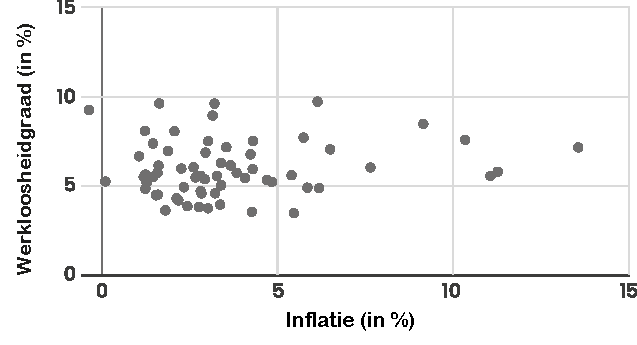
\includegraphics[width=\textwidth]{figures/fig1.pdf}
\caption[Relatie tussen werkloosheid en inflatie]{Relatie tussen werkloosheid en inflatie\index{inflatie}\footnotemark}
\label{fig1}
\end{figure}
\footautocite{11}


Ondanks decennia van opgestapeld bewijs dat het geen accurate verklaring is van hoe de wereld werkt, blijft deze theorie, tot op vandaag, echter bestaan. Rond 1970, toen wereldwijd zowel de inflatie\index{inflatie} als de werkloosheid toenamen, werd de Keynesiaanse trade-off zonder enige twijfel weerlegd. Maar het voordeel van economische wetenschap zonder systematische en herhaalbare methode van experimenteren en testen is dat theorieën na hun weerlegging altijd kunnen worden aangepast op een manier die afwijkende waarnemingen in de echte wereld goed praten. Dat is de essentie van pseudowetenschap.

Hilarisch genoeg pasten de Keynesianen hun theorie aan door er simpelweg een nieuwe term `aanbodschok' in op te nemen. Een aanbodschok is een onsamenhangende term, achteraf gemaakt als een rechtvaardiging om te verklaren hoe stijgingen in werkloosheid en inflatie\index{inflatie} tegelijkertijd kunnen voorkomen. Sindsdien zijn de wereldeconomieën getuige geweest van elke denkbare combinatie van inflatie\index{inflatie}- en werkloosheidscijfers, en de Keynesianen hebben met succes de waan in stand gehouden dat er zo’n trade-off tussen werkloosheid en inflatie\index{inflatie} bestaat. Elke afwijking van deze relatie kan worden verklaard door een aanbodschok of diverse andere denkbare substituten te hulp te roepen, en dus is er geen observatie mogelijk die deze relatie weerlegt. Het verklaart alles en verklaart daarom niets. De illusie van economie als een precieze, kwantitatieve en empirische wetenschap wordt alleen in stand gehouden door de theorieën vrij te stellen van empirisch onderzoek in de echte wereld.

\textbf{Na een eeuw natuurkunde te hebben nagebootst en klassieke methodologische grondslagen te hebben losgelaten, is de economie er niet in geslaagd om één kwantitatieve wet of formule te produceren die onafhankelijk getoetst en gerepliceerd kan worden.} Macro-economische formules komen en gaan met de modes van moderne ideologische stromingen, maar geen enkele is objectief gemeten en gerepliceerd op een manier waardoor het een wetenschappelijke wet genoemd kan worden. Dat macro-economie centrale regeringen macht geeft en academici verrijkt, kan helpen verklaren waarom het heeft standgehouden.

\section{Een contrast van benaderingen}

Om de benadering van het menselijk handelen\index{menselijk handelen} van de economische discipline te illustreren en te vergelijken met de moderne kwantitatieve economische methodologie, kunnen we als voorbeeld de kwestie van door de overheid\index{overheid} opgelegde minimumlonen nemen, die een ondergrens opleggen aan wat werkgevers hun werknemers kunnen betalen. Dit is een populaire beleidsinterventie in het grootste deel van de wereld, en de tegengestelde perspectieven hierop dienen als een les binnen de twee verschillende kaders voor het denken over economie: menselijk handelen\index{menselijk handelen} en aggregaten.

Stel je een politicus voor die verkiezingen wil winnen in een land zonder minimumloonwetten. Zoals in alle tijden en plaatsen in de menselijke geschiedenis is er een natuurlijke variatie in de lonen van arbeiders. De politica besluit haar campagne te richten op het verbeteren van de levensstandaard van de armsten uit de samenleving door een minimumloon te verplichten, waarvan ze zich voorstelt dat het de ontvangers ervan een fatsoenlijk bestaan garandeert. Op basis van haar macro-economische raamwerk dat gericht is op aggregaten, besluit de aspirant-leider een minimumloon van \$10 per uur op te leggen. De econoom concludeert dat 20\% van alle werknemers, die 35\% van de bevolking onderhouden, momenteel minder dan \$10 per uur verdienen. Het totale effect van het opleggen van het minimumloon zou leiden tot een loonstijging van \$10 miljard per jaar. Op basis van geavanceerde historische en theoretische modellen schat de econoom verder dat de stijging van de lonen met \$10 miljard zich zou vertalen in een stijging van de consumentenbestedingen met \$8 miljard, waarvan de modellen schatten dat dit zou resulteren in de creatie van 40.000 nieuwe banen, een stijging van de industriële productie\index{productie} met 12\%, een stijging van de export met 4\% en een stijging van het bruto binnenlands product met \$16 miljard.

Volgens deze collectivistische benadering van economische analyse zijn de aggregaten de causale factoren in economische fenomenen, en handelen ze volgens de theoretische relaties die door economen zijn vastgesteld, op een vergelijkbare manier als hoe natuurkundigen en scheikundigen wetenschappelijke regels vaststellen. Deze conclusies zijn tot stand gekomen met behulp van wetenschappelijk ogende vergelijkingen die niet veel verschillen van de vergelijkingen die gebruikt worden in de algemene gaswet. In het kader van de geaggregeerde economische analyse klinkt de wet op het minimumloon als een grote zegen voor de samenleving. De armste werknemers zullen hun levensstandaard aanzienlijk verhogen, sommige werklozen zullen werk vinden als gevolg van de extra uitgaven, en de hele samenleving wordt productiever. Bovendien stijgt de export, wat de economie aan buitenlandse valuta helpt.

Als dit te mooi klinkt om waar te zijn, dan is dat omdat het niet waar is. De dingen zien er anders uit door de lens van de econoom met de Mises-bril. De deugdelijke econoom weet dat menselijk handelen\index{menselijk handelen} de drijvende kracht achter menselijke zaken is en analyseert de wereld niet door middel van geaggregeerde grootheden. In plaats daarvan analyseert hij beslissingen van echte mensen die door deze nieuwe wet worden beïnvloed. Werkgelegenheid is een overeenkomst tussen twee individuen; de werkgever en de werknemer. Een deugdelijk econoom begrijpt dat de keuze van een ondernemer om iemand in dienst te nemen, gebaseerd is op een eenvoudige rekensom: hij zal hem in dienst nemen als zijn bijdrage aan de bedrijfsinkomsten groter is dan zijn loon. Als het wettelijk minimumloon hoger is dan de marginale opbrengst van de werknemer, dan kost het in dienst nemen van de werknemer het bedrijf\index{bedrijf} geld en is het een soort donatie van het bedrijf\index{bedrijf} aan de werknemer. Werkgevers weten dat het aannemen van zo’n werknemer een dure misstap is, en werkgevers die dat niet weten, zullen snel zien dat hun bedrijf\index{bedrijf} failliet\index{faillissement} gaat, omdat het geld blijft verspillen aan lonen die het zich niet kan veroorloven. Alleen werkgevers die deze economische realiteit begrijpen, zullen werkgevers blijven, en zij die dat niet doen, zullen hun bedrijf\index{bedrijf} verliezen. Emotionele chantage door politici kan niets aan deze realiteit veranderen.

Lonen zijn, net als alle prijzen op een markt, niet zomaar willekeurige getallen die door hebzuchtige werkgevers worden gekozen. Ze zijn een weerspiegeling van de marginale productiviteit van de werknemer. Nu de wet bepaalt dat een werknemer \$10 per uur moet krijgen, moet de werkgever opnieuw overwegen of het de moeite waard is om deze werknemer in dienst te nemen. Wanneer de overheid\index{overheid} een minimumloon oplegt, verandert dat niet op magische wijze de calculus van de werkgever, noch verhoogt het op magische wijze de productiviteit van de werknemer. De werkgever zal nog steeds alleen werknemers aannemen wiens productiviteit hoger is dan hun loon. De wet op het minimumloon maakt het dus illegaal voor werkgevers om iemand in dienst te nemen wiens marginale productiviteit minder is dan \$10 per uur. Elke werknemer met een lagere productiviteit zal nu een verlies betekenen voor elk bedrijf\index{bedrijf} dat hem in dienst neemt en hem dat bedrag betaalt. Of hij wordt ontslagen, of het bedrijf\index{bedrijf} dat hem inhuurt, verliest geld en gaat failliet\index{faillissement}. In alle gevallen worden deze banen geëlimineerd, en iedereen met een productiviteit van minder dan \$10 per uur is nu wettelijk werkloos; ofwel werkloos of illegaal tewerkgesteld.

Bekeken door de lens van menselijk handelen\index{menselijk handelen}, is het effect van een minimumloonwet dat het voor werknemers met een lage productiviteit illegaal wordt om een baan te krijgen, en veel van deze werknemers zullen hun baan verliezen. Als we verder kijken door de lens van menselijk handelen\index{menselijk handelen}, dan zien we dat de werknemers die hun baan verliezen de werknemers zijn met de laagste productiviteit in de samenleving, en dit zijn meestal de armste, jongste en minst ervaren werknemers. Door het voor hen illegaal te maken om te werken, wordt het voor hen in feite illegaal om hun productiviteit te verhogen door tijdens het werk te leren en waardevolle werkervaring op te doen. Minimumloonwetten zijn dus bijzonder schadelijk voor de mensen die het meest behoefte hebben aan werk, en ze zijn een factor die bijdraagt aan het ontstaan van grootschalige werkloosheid en ongeschiktheid voor de arbeidsmarkt. Een andere mogelijke implicatie is dat sommige bedrijven, vooral de bedrijven die voor hun bedrijfsvoering afhankelijk zijn van deze laagbetaalde arbeiders, hogere lonen zouden betalen, maar ook de prijzen van hun goederen zouden verhogen om de hogere lonen te financieren. Consumenten zouden dan de prijs\index{prijs} betalen door hogere productprijzen en een lagere hoeveelheid beschikbare goederen. In dit scenario wordt elke potentiële stijging van het inkomen van een werknemer met een laag loon tenietgedaan door een overeenkomstige stijging van de kosten van de goederen die hij moet consumeren.

Al deze gevolgen van minimumloonwetten zijn af te leiden door deugdelijke economen die de loonwet analyseren en de gevolgen ervan voor rationeel handelende individuen evalueren. Dit blijkt een veel nuttigere en nauwkeurigere beoordeling van de situatie te zijn dan alles wat we met wiskundige verhoudingen tevoorschijn kunnen toveren. Prijzen zijn een weerspiegeling van de onderliggende marktrealiteit die door menselijk handelen\index{menselijk handelen} wordt gestuurd. De onderliggende marktrealiteit veranderen door de weerspiegeling ervan te veranderen, werkt niet. Elke poging om prijscontroles door te voeren is mislukt omdat dit soort centrale planning de rol van menselijk handelen\index{menselijk handelen} negeert. Prijscontroles behandelen de economie alsof het over materiële objecten gaat, in plaats van menselijk handelen\index{menselijk handelen}. Schuettinger en Butler hebben een deprimerende, maar onderhoudende geschiedenis van prijscontroles geschreven in \textit{Forty Centuries of Price Controls}, waarin ze illustreren hoe deze exacte dynamiek zich in culturen en naties door de geschiedenis heen heeft herhaald.\autocite{12} Koningen, keizers, politici en bureaucraten zien de wereld van economische transacties als een onmenselijk proces dat ze naar gelang hun behoeften kunnen veranderen. Zij oordelen dat de waarneembare marktverschijnselen binnen aanvaardbare grenzen blijven. Ze gaan ervan uit dat mensen gewoon hun handelen zullen aanpassen om ervoor te zorgen dat deze wetten worden nageleefd. In werkelijkheid passen mensen hun handelingen aan om hun eigen welzijn te optimaliseren, niet om bureaucraten tevreden te stellen. De handelaar verkoopt liever helemaal niet dan met verlies. Je ziet ofwel de vrije marktprijs of je ziet helemaal geen marktprijs. In deze laatste economie komen echte prijzen tot stand op zwarte markten\index{markten}.

Deugende economen begrijpen dat waarneembare economische verschijnselen en statistieken slechts manifestaties zijn van het onderliggende handelen van de betrokken mensen. Mensen proberen voortdurend hun eigen levenssituatie te verbeteren en het is zinloos om hen te verplichten tegen hun eigen belangen in te handelen. Wetten opleggen die tegen het eigenbelang van mensen ingaan, verandert de menselijke natuur niet. Het vermindert de stimulans om zich legaal te gedragen en vernietigt zo het respect van de maatschappij voor wetten. Dit essentiële besef is de reden waarom de deugdelijke econoom voorstander is van individuele economische vrijheid en tegen de beperking ervan door overheden. De menselijke geest is ontembaar en zal niet handelen op een manier die schadelijk is voor zichzelf.

Een goede econoom begrijpt dat mensen voortdurend handelen om hun lot in het leven te verbeteren. Het opleggen van wettelijke straffen op elke vreedzame economische activiteit die ze zouden kunnen kiezen, kan niet leiden tot een verbetering van hun leven, omdat dit simpelweg de keuze aan handelingen die voor hen beschikbaar zijn, zal beperken en verkleinen.

Geaggregeerde analyse verblindt de nepeconoom voor de gevolgen van deze wetten voor de mensen wier vrijheden beperkt worden. Na het formuleren van wiskundige maatstaven voor sociale verschijnselen, neemt de collectivistische econoom vervolgens aan dat deze maatstaven oorzakelijke factoren zijn in het vaststellen van menselijke zaken.

De wereld heeft al veel te veel economische leerboeken die zijn geschreven in de pseudowetenschappelijke kwantitatieve traditie. Dit boek zal daar zeker niet bij horen. Het zal niet proberen om economie uit te leggen in de taal van de natuurwetenschappen, en het zal geen verfijnde aggregaatvergelijkingen bevatten. Dergelijke benaderingen beloven veel, maar leveren weinig betrouwbare, bruikbare inzichten op.
